\begin{comment}
    Use cases
    Multimodality

    Neural networks:
        Basics
        CNN
        U-NET

    Dataset

    Implementations:
        Colorful image colorization
        GAN/pix2pix
        IDeep
\end{comment}

\chapter{Base}
\label{ch:base}

The task of automatic colorization can be defined as an image-to-image 
translation problem \citep{pang2021imagetoimage}, where for a monochrome 
input image we have to propose a plausible colored output. Although 
grayscale is a subset of monochrome (meaning \textit{having one color}), 
the two terms will be used interchangeably throughout this thesis. 
The defining feature of the input images is that they only have one channel 
representing the perceptual lightness of the given image. That means that 
each pixel only has a numeric value, usually in the 8-bit range, 
expressing how light (or dark) it is. 

\begin{figure}[H]
    \centering
    \includegraphics[width=0.5\textwidth]{img/alim_khan.jpg}
    \caption{
    Colored image of Alim Khan taken by Sergey Prokudin-Gorsky 
    in 1911 using the three-image color photography method on the left,
    and the green, red, and blue (top to bottom) filter negatives
    (shown as positives) on the right.}
    \label{fig:alim_khan}
\end{figure}

On the other hand, if we want to render a colored photograph we need at 
least 3 channels to do so, meaning that for each pixel we want to draw, 
we need at least 3 values associated with it. The specific way of mapping 
the three values to a color is called a color space. An example of a color
space is the RGB color model in which each of the 3 channels depicts the 
amount of \textbf{R}ed, \textbf{G}reen, or \textbf{B}lue color present,
as shown in figure \ref{fig:alim_khan}. 

That said, the task of colorization can be summed up as
\begin{equation}
    \mathbf{Y} = \mathcal{F}(\mathbf{X})\;\mathbf{where}\;\;\mathbf{X} \in \mathbb{R}^{H \times W \times 1}, \mathbf{Y} \in \mathbb{R}^{H \times W \times 3}\label{eq:colorization}
\end{equation}    
where $\mathbf{X}$ is the input 
and $\mathbf{Y}$ is the colored output.
$\mathcal{F}$ is the function that maps the domain $\mathbf{X}$ to the codomain 
$\mathbf{Y}$, which in our case represents the colorizer.

\section{Color space}
\label{sec:colorspace}

Even though automatic colorization can be accomplished using any color space, 
as with any task some tools are better for the job than others. Although the 
RGB color space would be the easiest to use, as it is the default option for 
many tools, it doesn't give us an advantage when colorizing. On the other hand, 
the CIELAB color space has a few useful properties which make it convenient 
for the task. The CIELAB (or L*a*b*) color space was defined by the 
International Commission on Illumination in 1976 as an attempt to create a 
perceptually uniform color space \citep{icc2004cielab}. 
In perceptually uniform color spaces, a numeric change in any direction 
would result in a similar perceived color change. Although L*a*b* is not truly 
perceptually uniform, it is nevertheless useful for that purpose. Perceptual 
uniformity is not necessary while colorizing, but it is practical, as changes 
in value result in proportional color changes.

\begin{figure}[!h]
	\centering
	\begin{subfigure}{.24\textwidth}
		\centering
		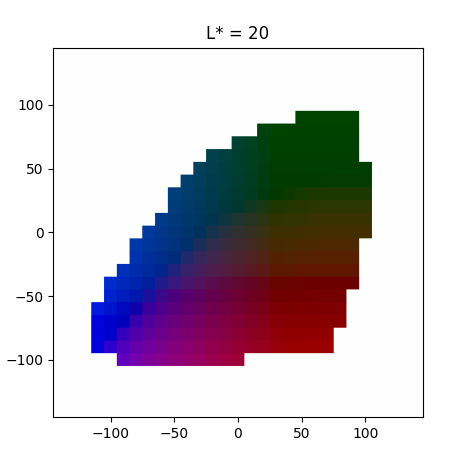
\includegraphics[width=\linewidth]{plot/lab/20}
	\end{subfigure}
	\begin{subfigure}{.24\textwidth}
		\centering
		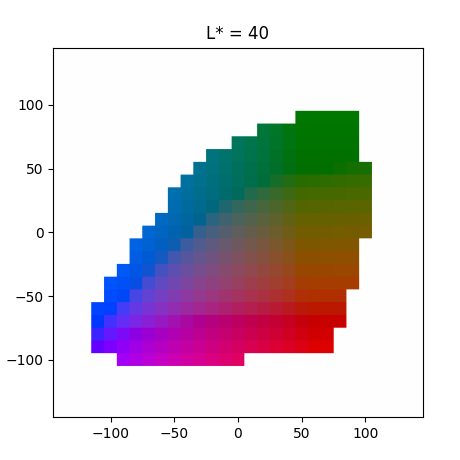
\includegraphics[width=\linewidth]{plot/lab/40}
	\end{subfigure}
	\begin{subfigure}{.24\textwidth}
		\centering
		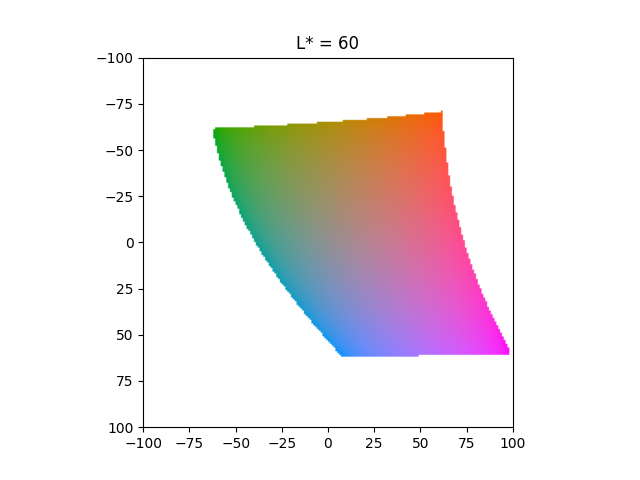
\includegraphics[width=\linewidth]{plot/lab/60}
	\end{subfigure}
	\begin{subfigure}{.24\textwidth}
		\centering
		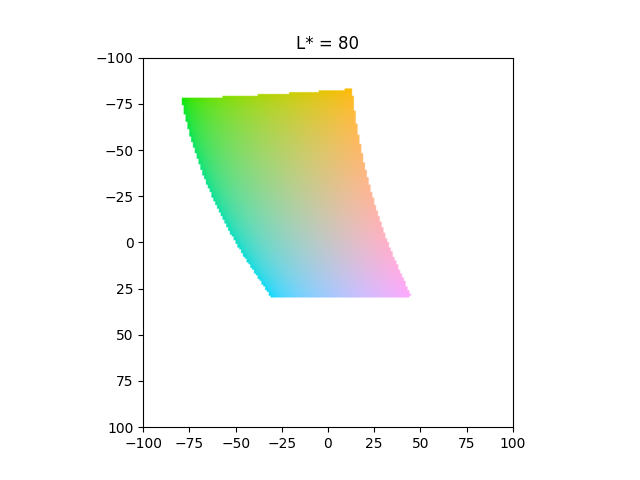
\includegraphics[width=\linewidth]{plot/lab/80}
	\end{subfigure}
    \caption{Slices of the CIELAB color space at different luminance levels, with only the RGB gamut rendered}
	\label{fig:rgb_in_lab}
\end{figure}

The CIELAB color space expresses colors using three channels. The bounded \textbf{L*}
channel is expressing the lightness of the color, with 0 representing black and 100 
white, respectively. The \textbf{a*} and \textbf{b*} channels, on the other hand, 
express the \textit{color}. Both color channels are unbounded, which allows the 
CIELAB color space to express the whole human gamut\footnote{The complete range 
or scope of something}. The RGB color space fits in the CIELAB color space 
as show in the figure \ref{fig:rgb_in_lab}.

\begin{figure}[!h]
	\centering
	\begin{subfigure}{.3\textwidth}
		\centering
		\includegraphics[width=\linewidth]{img/lab_channels/san_g}
        \caption{Original}
	\end{subfigure}
	\begin{subfigure}{.3\textwidth}
		\centering
		\includegraphics[width=\linewidth]{img/lab_channels/san_g_gs}
        \caption{\textbf{L*} channel}
	\end{subfigure}
	\begin{subfigure}{.3\textwidth}
		\centering
		\includegraphics[width=\linewidth]{img/lab_channels/san_g_color}
        \caption{\textbf{a*} and \textbf{b*} channels (\textbf{L*} = 75)}
	\end{subfigure}
    \caption{Image with seperated channels of the CIELAB color space}
	\label{fig:lab_channels}
\end{figure}

Another useful property of the CIELAB color space is that it has a dedicated channel
for perceptual luminance and two channels for the color, as seen in figure \ref{fig:lab_channels}. 
We can use that property for simplifying the process of colorization, as the input to the 
colorizer is the perceptual luminance of the grayscale image. That means that we only have to 
suggest the \textbf{a*} and \textbf{b*} (color) channels in order to colorize the image. 
That said, we can update the equation \ref{eq:colorization} to:
\begin{equation}
    \mathbf{Y} = \mathcal{F}(\mathbf{X})\;\mathbf{where}\;\;\mathbf{X} \in \mathbb{R}^{H \times W \times 1}, \mathbf{Y} \in \mathbb{R}^{H \times W \times 2}\label{eq:colorization_2}
\end{equation}    
as the colorizer only has to suggest two channels.

\section{Task definition}
\label{sec:task}

In the 2000s many algorithms for colorization were developed \citep{levin2004colorization}\citep{luan2007colorization}\citep{charpiat2008colorization}\citep{reinhard2001colorization} 
fueled by the ever growing computational capacaties of the modern world. Those were mostly 
statistical methods that relied on extensive user input to get a viable colorization. 
Nevertheless they offered a method for somewhat easy colorization that gave good results, 
but the problem of fully-automated image colorization still remained unsolved. A decade later 
first models \citep{cheng2015colorization}\citep{iizuka2016colorization} using the CNN
architecture started popping up, paveing the way for a fully-automated colorization process.
In this thesis three approaches to image colorization will lined out, all of which are using 
convolutional neural networks described in section \ref{sec:cnn}.


The goal for each of the models is to hallucinate a viable colorization for a grayscale 
input image. The colorizer has to propose the values for the \textbf{a*} and \textbf{b*}
channels, while the \textbf{L*} channel is the same as the input image. As noted in chapter \ref{ch:introduction}
perfect colorization is sometimes possible but highly unlikely, the goal is rather to 
produce a probable colorization which is able to fool human observers into thinking it is a 
real full-color image.

\subsection{Multimodality}
\label{sec:multimodality}

One of the reasons why perfect colorization is not possible has to do with the 
fact that a grayscale photograph has less information than a colored photograph.
Although it is sometimes possible to deduce exact colors from the shape or texture of
an object, more often than not we cannot be sure of the original color.
The problem becomes apperent when trying to colorize almost any painted object,
like the three scooters seen in figure \ref{fig:multimodality_scooters}. Given the 
grayscale image of the scooters one could assume that all of them are the same
color, which our colorizer did, or that they are all different colors, as seen 
in the original image. 

That fenomenon is not exclusive to human-made objects, 
but it also extends to the natural world as seen in the figure 
\ref{fig:multimodality_sunset}. In the grayscale image there is no clue to the 
fact that the picture was taken during a sunset, so the best the colorizer
was able to do was to colorize it as if it was an image of a stormy sea.

\begin{figure}
	\centering
	\begin{subfigure}{.32\textwidth}
		\centering
		\includegraphics[width=\linewidth]{img/multimodality/vespa_orig}
	\end{subfigure}
	\begin{subfigure}{.32\textwidth}
		\centering
		\includegraphics[width=\linewidth]{img/multimodality/vespa_gs}
	\end{subfigure}
    \begin{subfigure}{.32\textwidth}
		\centering
		\includegraphics[width=\linewidth]{img/multimodality/vespa_colorful}
	\end{subfigure}
    \caption{Image of three scooters, colorizer input, and possible colorization}
	\label{fig:multimodality_scooters}
\end{figure}

\begin{figure}
	\centering
	\begin{subfigure}{.32\textwidth}
		\centering
		\includegraphics[width=\linewidth]{img/multimodality/sunset}
	\end{subfigure}
	\begin{subfigure}{.32\textwidth}
		\centering
		\includegraphics[width=\linewidth]{img/multimodality/sunset_gs}
	\end{subfigure}
    \begin{subfigure}{.32\textwidth}
		\centering
		\includegraphics[width=\linewidth]{img/multimodality/sunset_colorized}
	\end{subfigure}
    \caption{Image of sea taken during a sunset, colorizer input, and possible colorization}
	\label{fig:multimodality_sunset}
\end{figure}

This occurs because it is impossible to create more information than there is present, 
but our model can try to find the most probable solution to the given problem and the context. 
Let's say we have a pair of two real positive numbers and the result of their 
addition is 4, our task is to find the values of the 2 numbers just knowing the 
result. The task seems impossible at first, as there is an infinite number of possible 
combinations that give the same result. But given the context that the pair was 
chosen by humans, and as humans like whole numbers, the chances of the pair being
$(1, 3)$ or $(2, 2)$ is much higher than for them to be $(3.141592, 0.858408)$. The posed
problem is quite similar to the task of colorization where the sum is the weighted 
average of the \textbf{R}, \textbf{G}, and \textbf{B} channels and the context is the 
whole image. As seen in the posed problem, there are several likely combinations
among the sea of unlikely ones. That property, where we have several possible modes 
or maxima is called multimodality, and it is the main problem when colorizing. It is
troublesome as we cannot be sure what the real solution is, but we can provide one 
of the multiple likely ones.

\section{Artificial neural networks}

\begin{figure}
	\centering
	\begin{subfigure}{.49\textwidth}
		\centering
		\includegraphics[height=.52\linewidth]{img/neuron}
	\end{subfigure}
	\begin{subfigure}{.49\textwidth}
		\centering
		\includegraphics[height=.52\linewidth]{img/simple_nn}
	\end{subfigure}
    \caption{Comparison of biological and artificial neuron (stronger colors indicate higher weights)}
	\label{fig:neuron}
\end{figure}

Artificial neural networks, or simply called neural networks in the context of 
machine learning, are a class of highly versatile computational models used for 
regression, classification, data processing, etc. As with many successful computational 
systems, artificial neural networks are vaguely inspired by real-world examples,
in this case, biological neural networks, as seen in figure \ref{fig:neuron}. 

In simple, single-layer neural networks like the one seen in figure \ref{fig:neuron}, 
it is possible to understand how the model is working based on the weights it gives
to different inputs for different outputs. With deep, multi-layer neural networks 
we lose that \textit{interpretability}, as we give the neural network the possibility
to divide the problem into several layers of understanding which are virtually 
impossible to decipher. The learning part of machine learning takes place during the
training process, and is out of the scope of this thesis.

\subsection{Convolutional neural networks}
\label{sec:cnn}

Like neural networks, convolutional neural networks (or CNNs) were originally 
nature-inspired, specifically by the way that the animal visual cortex is 
organized \citep{fukushima1980neocognitron}. Instead of associating specific
inputs with specific weights, with CNNs we train the network to learn filters 
(or kernels) that we slide over features to get feature maps. When we stack
several convolutional layers on top of each other we get a deep convolutional
neural network (or DCNN). As with deep neural networks, the stacking allows 
the DCNNs to divide the problem into several layers of understanding. 

Let's say we have a picture of nature and we want to detect trees. A potential 
kernel would have the shape of a leaf, so when the kernel slides over a leaf on
the image, it activates. As the result of sliding over the whole image, we would
get a feature map where we know the positions of all leaves. In the next layer, 
the CNN could look for a canopy-shaped cluster of leaves. When it slides
over such a part of the feature map, it activates and at that point, we know the position
of the canopy.

Of course, that explanation is oversimplified, but it explains a possible way 
that a CNN deduces where a tree is. In reality, a leaf-shaped kernel will almost
certainly not happen, as kernels are usually much smaller in size (models
described in this thesis use $3\times3$ and $4\times4$ kernels), just enough to 
detect edges. Using the information about the relative position of different edges
from the first feature map, higher levels of abstraction should be achievable in 
subsequent layers. So while a leaf detecting kernel is improbable, within a couple
of layers the same level of \textit{understanding} can be achieved.

\subsection{U-net}

\begin{figure}[!h]
	\centering
	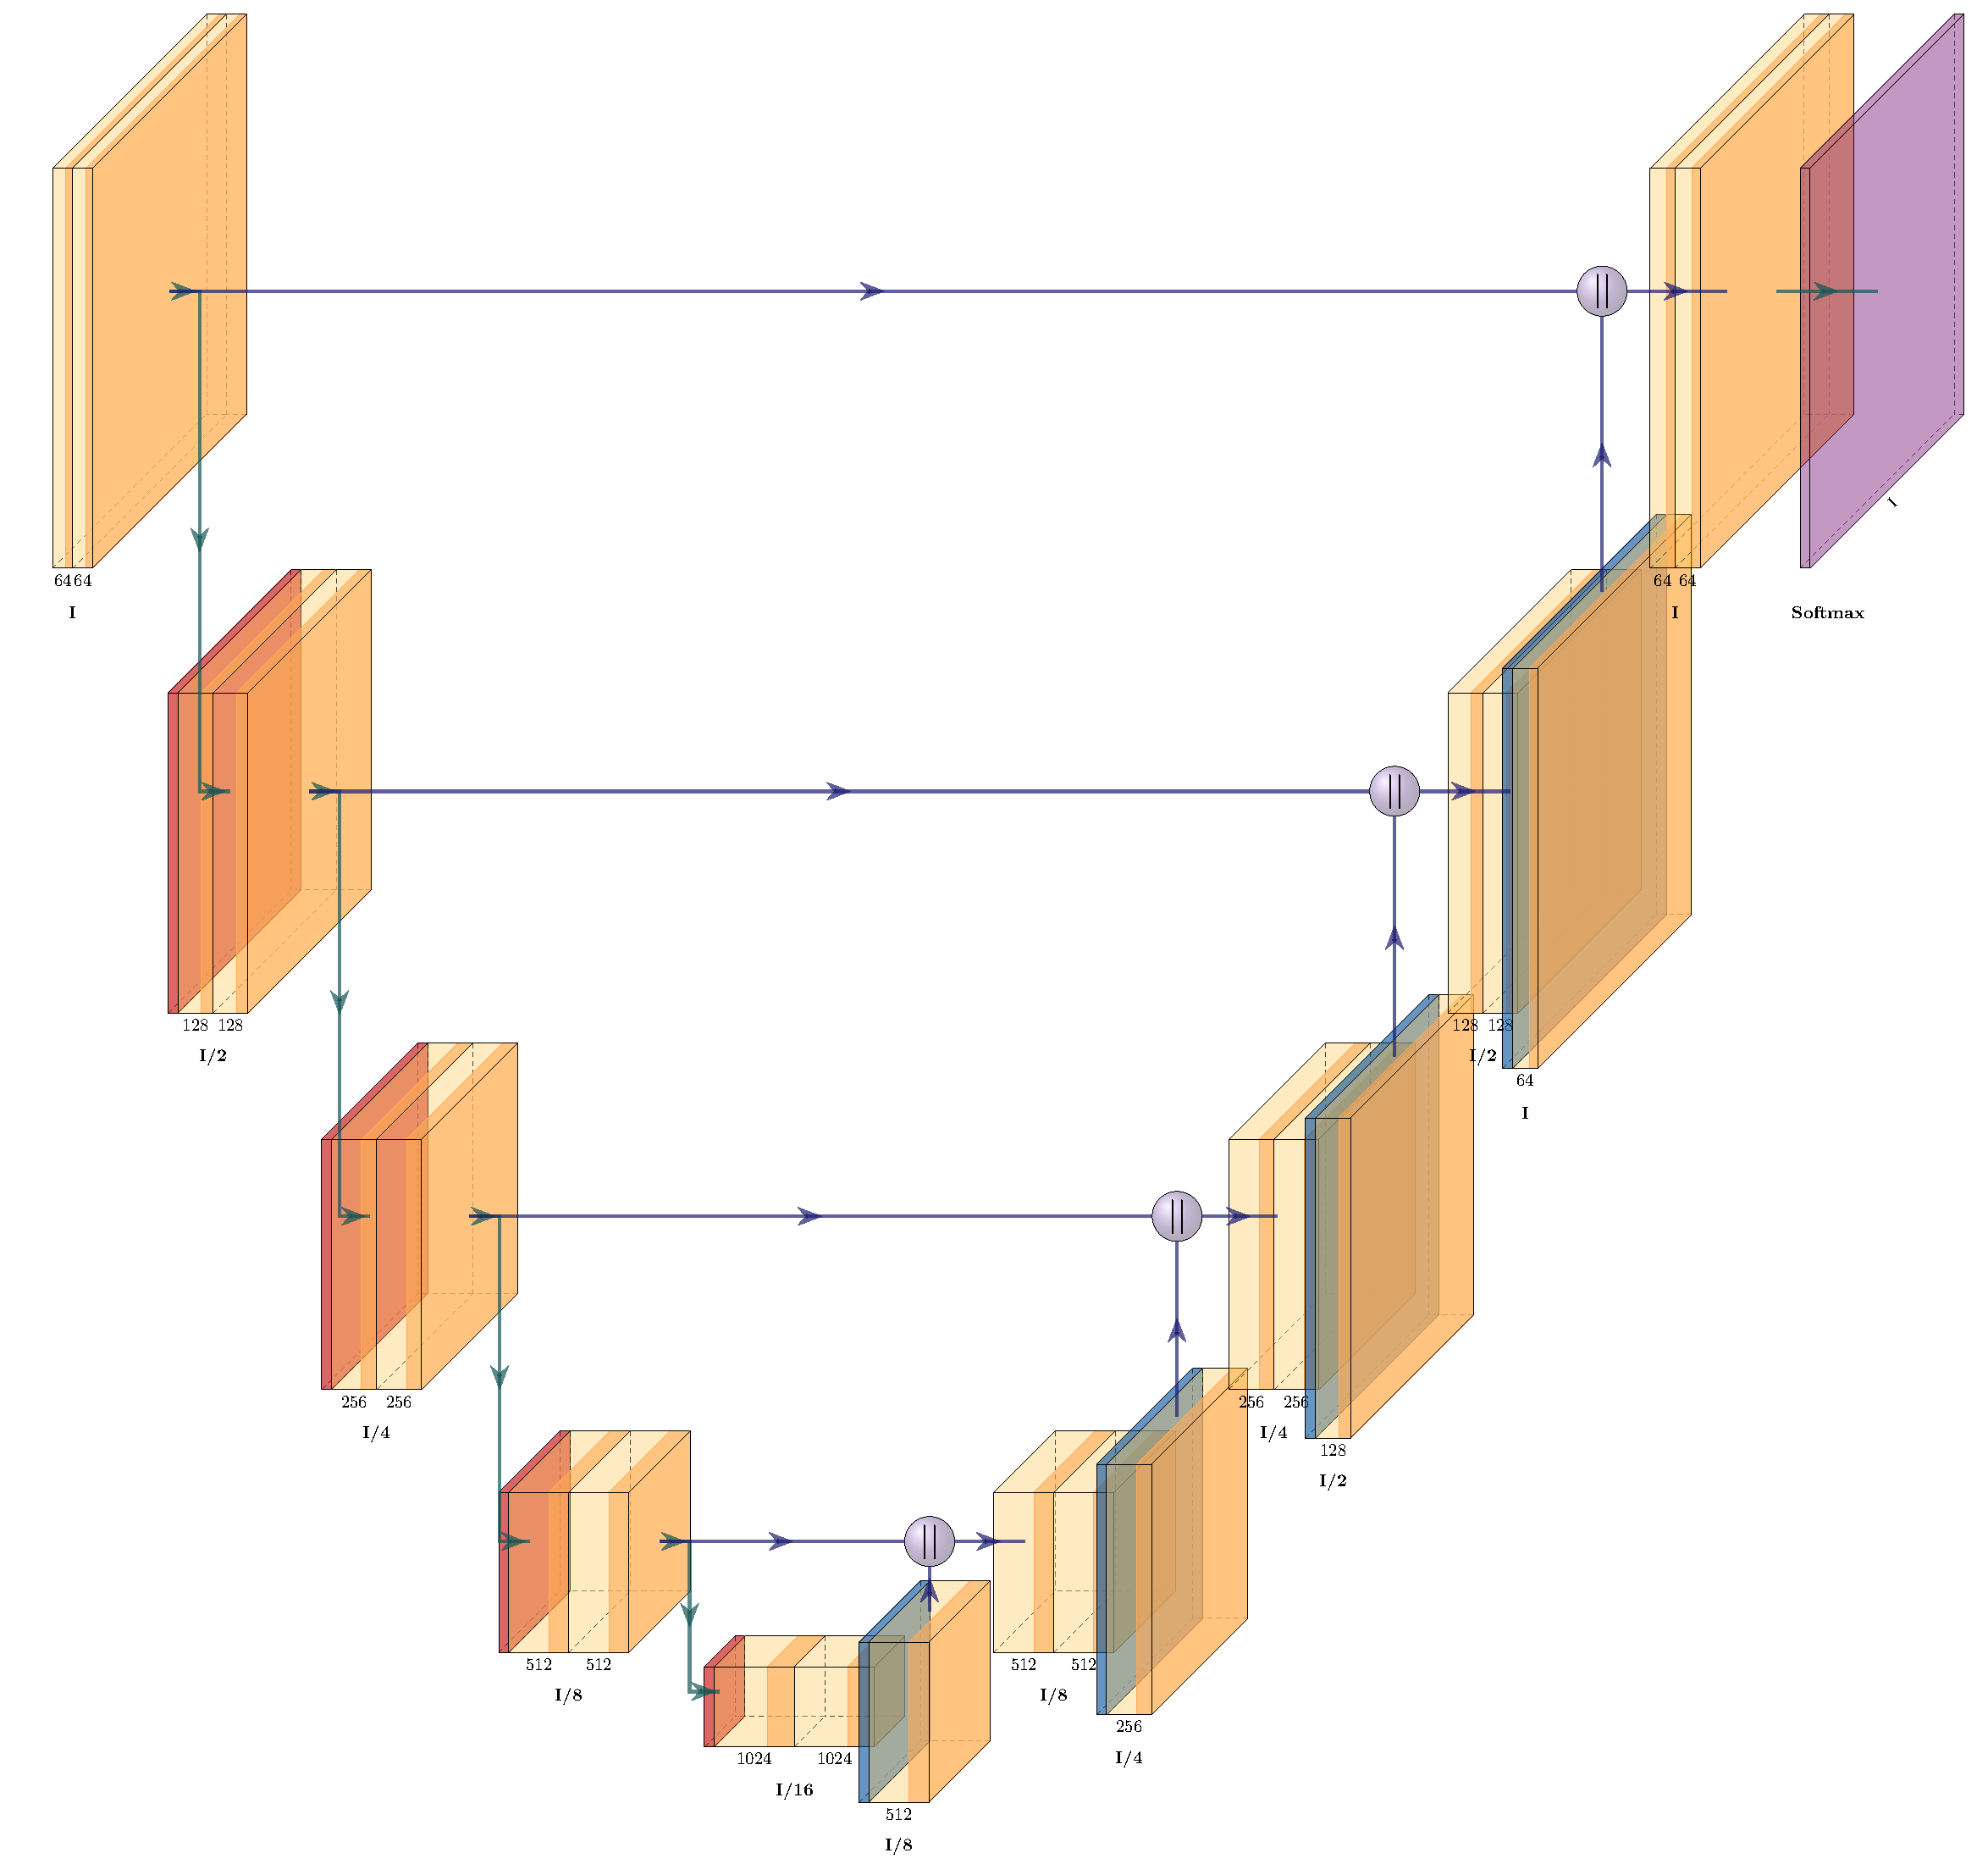
\includegraphics[width=0.65\linewidth]{architecture/unet}
    \caption{Example of a U-Net with four downsampling and four upsampling blocks 
	where the skip-connection is accomplished by concatinating outputs of the 
	encoder to the upsampled features of the decoder}
	\label{fig:unet}
\end{figure}

One specialized version of a deep convolutional neural network is the U-Net 
architecture which belongs to the class of fully convolutional neural networks. 
Originally designed for segmentation in the biomedical field, due to the ease
of training and the quality of the results, it has found use in many other 
image processing tasks. It owes its name to the usual way the network is 
visualized as seen in figure \ref{fig:unet}.

The network consists of symmetrical contractive and expansive paths, that are also
called the encoder and decoder respectively. Information is extracted from
the input and condensed in the encoder part of the network. At the end of the 
encoder, we find the narrowest part of the network that is also the bottleneck 
of the system. Although there is loads of information, if we upsampled at that 
point only using the features available in the bottleneck, the decoder might
not have some clues that were lost while downsampling. That problem is 
solved by adding skip connections from convolutional blocks in the encoder to
the corresponding blocks in the decoder as seen in the diagram \ref{fig:unet}. 
There are different ways of implementing skip connections, with the default one
being simple concatenation. 

\section{Dataset}
\label{sec:dataset}

Besides the network architecture, another crucial part that determines the quality
of the final product is the data on which the network was trained. If we have bad
data we can expect bad results, as the network will try to reproduce what is learned.
So for example, if we train the model on color-negatives we cannot expect that 
our model will colorize correctly, quite the opposite is true as the model will
try to reproduce what it has already seen. 

The database used for training all the architectures described in this thesis is 
the ImageNet database \citep{deng2009imagenet}. At the time of writing, it 
consists of 1.3 million images ordered in 1000 categories. The database is used 
as it covers a broad spectrum of different objects, animals, and places from all 
around the world. That versatility is desirable as our network has to \textit{see}
as many different things as it is possible, as it cannot know how to colorize something 
it has not come in contact with.

Any large collection of images, such as the Caltech 101 \citep{fei2004caltech}, 
Places \citep{zhou2017places}, or Cifar100\citep{krizhevskycifar} dataset, 
could have been used for training the models. We do not need a specialized dataset, 
as we can create our input grayscale images using the original colored images.
The only requirement is that the dataset covers a large spectrum of different
situations. A model trained on a dataset containing only images of nature 
would hardly know what to do when it receives a car as an input.

The only preprocessing step we have to do with the dataset is to remove noisy data, 
which in our case were the monochrome images in the dataset. About one-tenth of 
the ImageNet dataset was grayscale. The grayscale images were filtered out by 
first converting the image to the L*a*b* color space, and then checking if all 
the pixel values were within a radius around $(0, 0)$ which represents a shade of grey. 

The problem with this method is that it only removes truly grayscale images while
it leaves sepia and other monochrome images in the database. That problem could 
be solved by calculating the average color of the whole image, and instead of
checking if every pixel is close to $(0, 0)$, we could check if it was close
to the average color of the image. That way all images that consist only of 
different shades of the same color would be filtered out.
